\chapter{Simulation des robots}
\chaptermark{Robots}
\label{chapitre:robots}
	
	\section{Introduction}

		L'environnement dans lequel doivent évoluer les robots à été défini dans le \textsc{Chapitre}~\ref{chapitre:environnement}. Il est maintenant temps de simuler les \gls{ROV}s. Pour ce faire, nous allons devoir décrire les paramètres mécaniques des robots \argos{} et \atoll{}, et décrire le comportement de leurs capteurs et actionneurs à simuler. A la fin de cette partie nous devrions être en mesure de pleinement simuler les robots dans leur environnement, et le simulateur complet devrait ainsi respecter toutes les exigences présentées dans le \textsc{Chapitre}~\ref{chapitre:systeme}.

	\section{Simulation des composants}

		\subsection{Composition des robots}
			En remarquant que les deux robots embarquent un certain nombre d'éléments communs, il est possible de definir et de simuler ces différents composants dans \gazebo, afin d'être par la suite chargés dans la simulation des deux robots. La \textsc{table}~\ref{table:components} présente les différents composants à simuler et les dépendances entre les robots et les composants. On y retrouve aussi s'ils nécéssitent l'utilisation d'un \plugin{} \gazebo{} pour décrire leur comportement et d'une \gls{HardwareInterface} pour s'interfacer avec le reste de l'implémentation logicielle.

		\begin{table}[!htb]
			\centering
			\begin{adjustbox}{max width=\textwidth}
				\begin{tabular}{|l|c|c|c|c|}
					\hline
					Composant & \argos{} & \atoll{} & \gls{HardwareInterface} & \gazebo{} \plugin{} \\
					\hline
					Chassis d'\argos{} & \cmark & \xmark & \xmark & \xmark \\
					\hline
					Chassis d'\atoll{} & \xmark & \cmark & \xmark & \xmark \\
					\hline
					Boîtier electronique & \cmark & \cmark & \xmark & \xmark \\
					\hline
					Crochet de levage & \xmark & \cmark & \cmark & \cmark \\
					\hline
					Caméra de navigation & \cmark & \cmark & \xmark & \cmark \\
					\hline
					Caméra d'observation & \cmark & \cmark & \xmark & \cmark \\
					\hline
					Centrale Inertielle & \cmark & \cmark & \xmark & \cmark \\
					\hline
					Lumières étanches & \cmark & \cmark  & \cmark & \cmark \\
					\hline
					Propulseur & \cmark & \cmark & \cmark & \cmark \\
					\hline
					Nacelle pour caméra & \cmark & \cmark & \cmark & \cmark \\
					\hline
				\end{tabular}}
			\end{adjustbox}
			\caption{Composants à simuler}
			\label{table:components}
		\end{table}

		\subsection{Séparation en paquets}

			La convention \gls{ROS2} et \gazebo{} pour la description des robots prévoit de répartir le code dans différents paquets. Nous allons appliquer ici cette même convention pour chaque composant à simuler. Pour un composant s'appellant \textit{composant}, nous aurons les paquets suivants :

			\begin{itemize}
				\renewcommand{\labelitemi}{\textbullet}
				\item \textbf{composant\_description} :
				\begin{itemize}[noitemsep]
					\item Description URDF comportant les couches visuelles, inertielles et de collision
					\item Maillages 3D permettant de représenter visuellement le composant
					\item Fichier de configuration pour visualiser le composant dans RViz2
				\end{itemize}
				\item \textbf{composant\_gazebo} :
				\begin{itemize}[noitemsep]
					\item \textit{Plugin} décrivant le comportement du composant dans \gazebo{}
					\item Ficher de lancement du composant dans \gazebo{}
				\end{itemize}
			\end{itemize}

		Nous allons à présent détailler l'implémentation réalisée pour simuler ces composants.

		\subsection{Implémentation des composants}

			\subsubsection{Latch}

				Le \textit{Latch} est un composant propre au robot \gls{Atoll}. Ce crochet de levage permettant de transporter des structures sous-marines pouvant peser jusqu'à $1,5\ T$ est fabriqué par Forssea Robotics, et permet de positionner et de transporter des balises de positionnement acoustique sur les fonds marins.

				L'architecture logicielle du \textit{Latch} est présentée en \textsc{Figure}~\ref{fig:sa_latch}. Le composant reçoit deux informations de la part de l'implémentation logicielle : s'il est alimenté via le canal de communication \textit{power} et le signal de relâchement du crochet sur le canal \textit{release}. En retour, le crochet de levage renvoit son état à l'aide d'une sonde à effet hall qui indique si le crochet est fermé ou ouvert sur le canal \textit{sensor}.

				\begin{figure}[!htb]
					\centering
					\includegraphics[]{imgs/components/sa_latch.pdf}
					\caption{Architecture logicielle du \textit{Latch}}
					\label{fig:sa_latch}
				\end{figure}
							
				Le \plugin{} \gazebo{} développé afin de décrire le comportement du \textit{Latch} est basé sur la machine à états finis présenté en \textsc{Figure}~\ref{fig:latch_fsm}. L'idée est de créer une liaison encastrement dynamique entre le \textit{Latch} et la structure sous-marine à transporter. La logique implémentée dans la machine à état finis permet de simuler le fait que mécaniquement le crochet s'accroche automatiquement à un point d'attache de structure sous-marine qui rentrerait dans le composant, et que l'on ne commande que le relachement de cette structure par l'ouverture du crochet.

				\begin{figure}[!htb]
					\centering
					\includegraphics[scale=0.8]{imgs/latch_fsm.pdf}
					\caption{Machine à états du \textit{Latch}}
					\label{fig:latch_fsm}
				\end{figure}

				On obtient alors le composant simulable dans l'environnement de simulation \gazebo{} et visualisable dans \rviz{} comme on peut le voir sur la \textsc{Figure}~\ref{fig:latch_gazebo_rviz}.

				\begin{figure}[!htb]
					\centering
					\caption{Simulation du Latch}
					\label{fig:latch_gazebo_rviz}
				\end{figure}
		
			\subsubsection{SS309 Tilt}

				Le \textit{SS309 Tilt} est un composant commercialisé par l'entreprise \textit{Sidus Solutions} et qui permet dans les \gls{ROV}s d'orienter la caméra d'observation. Il est parfaitement étanche et comporte un jeu d'engrenages reliés à un moteur pas-à-pas pilotable en vitesse et en position. On demande ainsi au moteur de mettre l'axe à une certaine position, et l'axe se déplace avec une vitesse de rotation spécifiée.
			
				Pour simuler cet aspect pilotable en vitesse de rotation et position, il faut passer par la simulation d'un moteur pas-à-pas. C'est un moteur un moteur composé de plusieurs bobinages créant ainsi plusieurs phases qui sont allumées succéssivement afin de réaliser une rotation de l'arbre moteur d'un certain incrément d'angle. Cet angle est défini par les caractéristiques du bobinage et n'est donc pas réglable. Il n'est pas non plus possible de piloter précisement la vitesse avec laquelle il se rend à cette position incrémentée. En revanche, il est tout à fait possible de connaître précisement la position du moteur, car l'arbre moteur ne peut prendre qu'un nombre fini d'angles, et il suffit donc de compter le nombre d'incréments commandés. Enfin, on peut commander la vitesse avec laquelle le moteur se rend à cette position, en allumant les phases à la vitesse désirée.

				L'architecture logicielle du \textit{SS309 Tilt} est présentée en \textsc{Figure}~\ref{fig:sa_tilt}. Le composant reçoit de la part de l'implémentation logicielle s'il est alimenté via le canal de communication \textit{power}, ainsi que la position et la vitesse consigne sur les canaux \textit{command/position} et \textit{command/velociy}.Il renvoit sa position et sa vitesse réelle récupérée dans l'environnement de simulation sur les canaux \textit{state/position} et \textit{state/velociy}.

				\begin{figure}[!htb]
					\centering
					\includegraphics[]{imgs/components/sa_tilt.pdf}
					\caption{Architecture logicielle de la nacelle de caméra}
					\label{fig:sa_tilt}
				\end{figure}

				Nous allons à présent distinguer la position réelle de l'arbre moteur, la position cible et la position commandée. La position réelle est la position de l'arbre moteur dans le simulateur. La position cible est un multiple de l'incrément d'angle à laquelle doit se rendre le moteur à l'instant actuel. La position commandée la position finale dans laquelle doit se retrouver l'arbre moteur et peut être une position réelle quelconque. Le moteur ne sera capable que de se rendre à la position multiple de la valeur de l'incrément d'angle la plus proche de la position commandée. La \textsc{Figure}~\ref{fig:tilt_position} reprends ces différentes notions. En commandant la vitesse à laquelle on incrémente la position cible, on contrôle l'axe en vitesse.

				\begin{figure}[!htb]
					\centering
					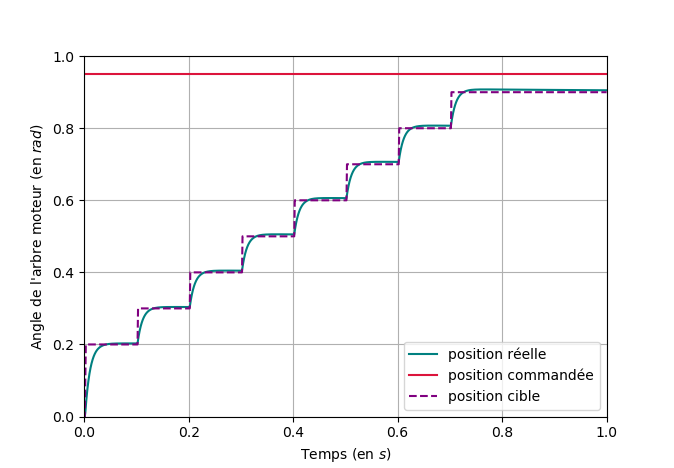
\includegraphics[width=0.6\textwidth]{imgs/stepper_motor.png}
					\caption{Simulation d'un moteur pas-à-pas}
					\label{fig:tilt_position}
				\end{figure}
				
				Pour ce qui est de l'implémentation de ce comportement dans \gazebo{}, on crée un \textit{Thread} qui va s'executer en boucle avec une vitesse variable. Cette vitesse sera fonction de la vitesse de commande du \textit{Tilt} notée $\omega_c$. A chaque tour de boucle, on incrémente donc la position cible de la valeur de l'incrément $d\theta$ si la différence entre la position réelle et la position commandée est plus grande que ce même incrément, et on attends le temps $h$, avec :

				$$h = \frac{d\theta}{\omega_c}$$

				\begin{algorithm}[!htb]
					\caption{Algorithme de simulation d'un moteur pas-à-pas}
					\label{algo:stepper_motor}
					\begin{algorithmic}
						\WHILE {true}
							\STATE read $\theta_r$, $\omega_c$
							\IF {$|\theta_c - \theta_r| > d\theta$}
								\STATE $\theta_t \leftarrow \theta_t + d\theta$
							\ENDIF
							\STATE $h \leftarrow \frac{d\theta}{\omega_c}$
							\STATE sleep $h$
						\ENDWHILE
					\end{algorithmic}
				\end{algorithm}

			\subsubsection{SPE75 Thrusters}

				\subsubsubsection{Présentation}
		
					Les \textit{SPE75 Thrusters} sont les propulseurs qui permettent aux robots de se déplacer et de s'orienter dans leur environnements. Ils sont composés d'un moteur permettant de mettre en mouvement des pale qui va permettre de générer une force dans la direction du propulseur.
					
				\subsubsubsection{Hardware Interface}

					L'\textit{Hardware Interface} va proposer une interface aux contrôleurs permettant d'appliquer une force suivant l'axe du propulseur qui va être transmise au robot. Elle va ensuite se charger de calculer la vitesse de rotation des pales nécéssaire à la création de cette force. Pour le composant réel, cette vitesse va être transmise au propulseur qui générer la force voulue et un couple résistant dans le sens inverse de la rotation des pâles sur le corps du propulseur qui va être transmis au robot. Pour le composant simulé, on est en mesure d'intéragir avec le simulateur afin d'appliquer des forces et des couples directement sur les objets simulés. 
					
					Le calcul de la vitesse de rotation des pâles en fonction de la force demandée est réalisé grâce à une interpolation de points de mesures faits sur un banc d'essai. L'idée est de faire tourner en eau le propulseur fixé sur un capteur de force à une certaine vitesse, et de mesurer la force générée par celui-ci. Ensuite, on est capable d'interpoler les pointsexpérimentaux logiciellement à l'aide de la librairie \gls{GSL}\footnote{\url{https://www.gnu.org/software/gsl/}} et de la fonctionnalité \textit{spline}. On peut ainsi calculer une vitesse de rotation à appliquer quel que soit la valeur de force demandée.
					
					L'idée retenue pour ce simulateur est d'appliquer directement la force demandée sur le corps du propulseur, car il est assez difficile et coûteux en ressources de calculs de realiser de la mécanique des fluides afin de simuler pleinement le comportement des pâles du propulseur. Il est tout de même nécéssaire de faire tourner les pâles dans le simulateur, car outre l'aspect cosmétique de voir les pales tourner quand le moteur fournit une poussée au robot, le simple fait de faire tourner ce solide ayant une certaine masse dans le simulateur va générer le couple résistant sur le corps du propulseur. Ainsi cette \textit{Hardware Interface} va communiquer au \textit{Model Plugin} la force et la vitesse de rotation des pâles calculée à appliquer sur le propulseur simulé.
		
				\subsubsubsection{Model Plugin}

					Le \textit{Model Plugin} va se charger d'appliquer la force et la vitesse de rotation communiquée par l'\textit{Hardware Interface}. Le \textit{plugin} est chargé pour chaque propulseur simulé et permet d'accéder finement aux paramètres de la simulation. On peut alors appliquer à chaque incrément de simulation la force demandée sur le corps du propulseur et la vitesse de rotation sur la liaison pivot entre le corps du propulseur et les pâles.

	\section{Simulation d'\argos{}}

	\section{Simulation d'\atoll{}}

	\section{Conclusion}